%%
% 引言
% 引言是论文正文的开端,应包括毕业论文选题的背景、目的和意义;对国内外研究现状和相关领域中已有的研究成果的简要评述;介绍本项研究工作研究设想、研究方法或实验设计、理论依据或实验基础;涉及范围和预期结果等。要求言简意赅,注意不要与摘要雷同或成为摘要的注解。
%%

\chapter{引言}
\label{cha:introduction}

\section{问题背景}
\label{sec:background}
% What is the problem
% why is it interesting and important
% Why is it hards, why do naive approaches fails
% why hasn't it been solved before
% what are the key components of my approach and results, also include any specific limitations,do not repeat the abstract
%contribution

强化学习(Reinforcement Learning, RL)\cite{ReinforcementLearning2021} \cite{suttonReinforcementLearningIntroduction2018} 是机器学习(Machine Learning,  ML)领域的一部分。不同于监督学习,强化学习不需要带标签的学习样本, 而是利用奖励或惩罚智能体行为的方式间接设定学习目标。 RL 的灵感 \cite{ReinforcementLearning2021} 来源于心理学中的行为主义理论,即有机体如何在环境给予的奖励或惩罚的刺激下,逐步形成对刺激的预期,产生能获得最大利益的习惯性行为。理论上,强化学习可以达到人工智能(Artificial General Intelligence, AGI)\cite{salvadorREINFORCEMENTLEARNINGLITERATURE2020}。

在标准的强化学习 \cite{mnihAsynchronousMethodsDeep2016} 中,有几个重要的概念:智能体(agent),环境(environment),状态(state),动作(action)和奖励(reward)。考虑扫地机器人的场景:机器人通过在房间里移动和执行清扫动作,从而完成任务。如果有多个扫地机器人,如何挑选出“最好”的一个呢?我们可以计算每块地砖的清洁程度,设定合理的评分机制,从而挑选出得分最高的扫地机器人出来。如果从强化学习的角度看待这个问题,扫地机器人是智能体,房间里面的所有事物就是智能体所在的环境,智能体所在位置以及房间的形状、清洁程度就是改环境的状态,移动和执行清理动作是动作,而每块砖的清洁程度的增加量就是奖励,只是我们要训练出一个得分高的扫地机器人,而不是挑选出一个。现实中有很多这样的问题场景,例如棋盘游戏、电子游戏和自动驾驶等。我们抽象出强化学习的理论框架\cite{suttonReinforcementLearningIntroduction2018}:智能体是完成任务的机器,它负责学习和决策,而智能体执行任务过程中应对的外部事物是环境。这些事务之间持续进行交互,智能体选择动作,环境对这些动作做出响应,呈现出新的状态。同时智能体获取一个奖励,智能体的目标是最大化总的奖励。图 \ref{fig:agent-env-interaction} 展示了整个交互的过程,这将在第二章继续讨论。


\begin{figure}[h]
	\centering
	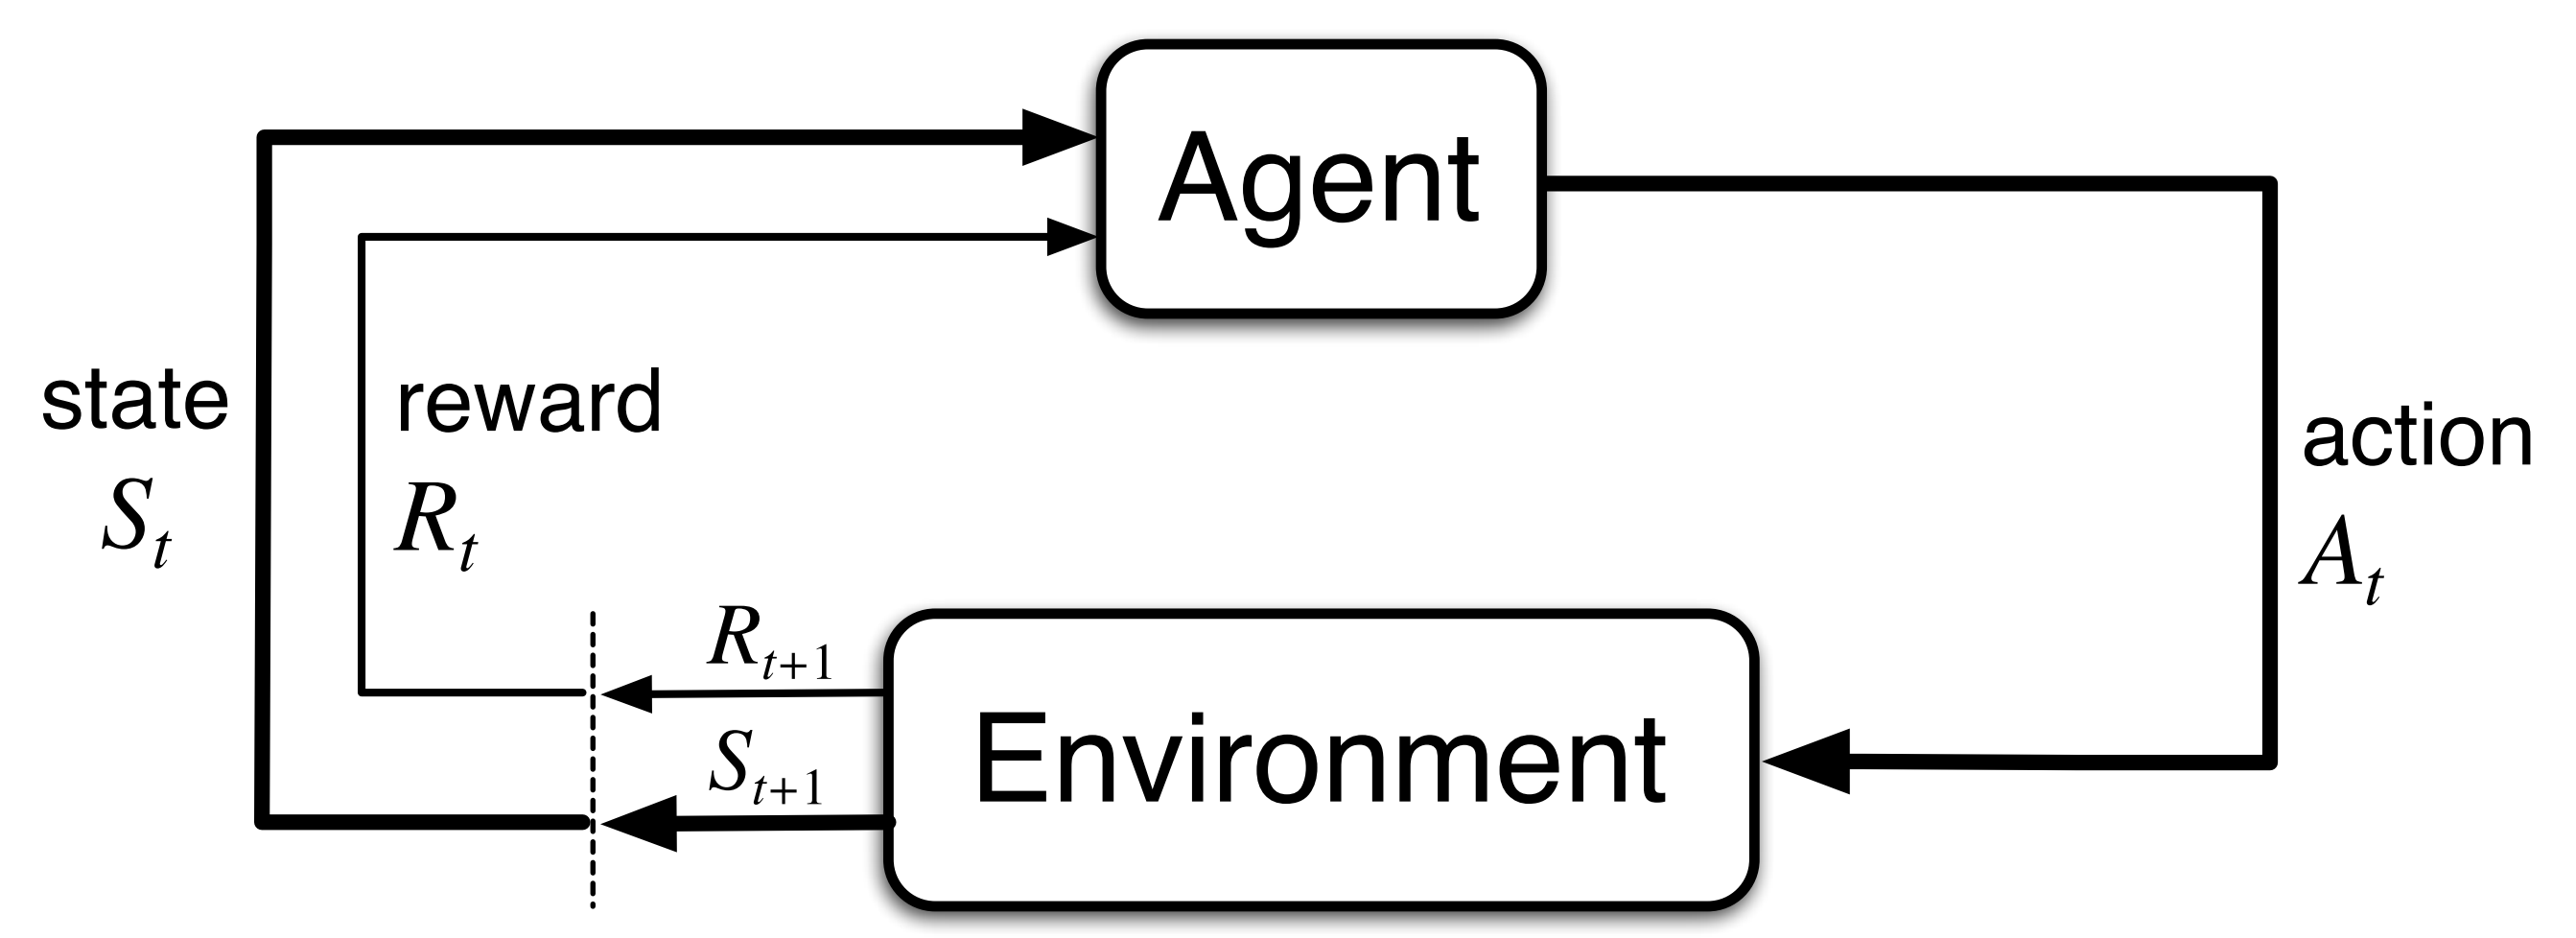
\includegraphics[width=0.9\textwidth]{image/chap01/interaction.png}
	\caption{智能体与环境交互过程\cite{suttonReinforcementLearningIntroduction2018}}
 	\label{fig:agent-env-interaction}
\end{figure}

% \section{强化学习介绍}
在上个世纪,对强化学习的研究已经有很多重要的理论和实践的成果出现\cite{suttonReinforcementLearningIntroduction2018}。过去的强化学习算法主要分为两类,以Q学习\cite{watkinsQlearning1992}算法为代表的基于值函数的方法和以策略梯度\cite{mnihAsynchronousMethodsDeep2016}算法为代表的基于策略的方法。
近些年来,由于深度学习技术的兴起,强化学习的研究和应用上取得巨大的成就。Mnih 等人提出了DQN 算法\cite{mnihPlayingAtariDeep2013} \cite{mnihHumanlevelControlDeep2015},该算法结合深度学习技术与经典的Q学习算法 \cite{watkinsQlearning1992},使得智能体在 Atari 类游戏能达到人类的控制水平。当然,RL中最令人兴奋的成功案例之一是DeepMind公司开发的AlphaGo \cite{silverMasteringGameGo2016} 和AlphaZero \cite{silverMasteringGameGo2017} 围棋程序。AlphaZero可以玩国际象棋,围棋和其他游戏,相对于仅玩围棋的AlphaGo,它在性能和通用性方面都有改进。这些程序在其他几个方面也很出色。特别是,他们学会了如何在没有人工指导的情况下学会玩游戏。

大部分最近的强化学习相关工作并没有完全脱离原来的研究成果,而是以过去的研究所得的结论为理论基础的 \cite{ohDiscoveringReinforcementLearning2020}。然而,强化学习实践上许多棘手的问题例如稀疏奖励、不完全的状态观察、学习样本不够等等,在根据理想假设的理论上设计的基于值函数或者基于策略的方法并不能很好地解决。本文探索在这些算法的基础上,能否通过机器自动学习到更加适合问题的强化学习算法。


\section{本文的论文结构与章节安排}
\label{sec:arrangement}

本文共分为六章,各章节内容安排如下:第一章提出文章的问题背景,同时介绍强化学习的作用和相关进展。 第二章是背景知识,介绍理解强化学习各个算法所必需的知识点。第三章是文献综述,对与本文方法相关的文献进行整理。第四章是本文算法的详细描述,同时穿插着作者的考量。第五章是本文所提出的方法的实验验证,将本文方法与经典的算法进行对比,然后分析实验结果。第六章总结本文所有的工作,指出本文方法的优点和不足之处,并提出可能做的改进。
